% ****** Start of file aipsamp.tex ******
%
%   This file is part of the AIP files in the AIP distribution for REVTeX 4.
%   Version 4.1 of REVTeX, October 2009
%
%   Copyright (c) 2009 American Institute of Physics.
%
%   See the AIP README file for restrictions and more information.
%
% TeX'ing this file requires that you have AMS-LaTeX 2.0 installed
% as well as the rest of the prerequisites for REVTeX 4.1
% 
% It also requires running BibTeX. The commands are as follows:
%
%  1)  latex  aipsamp
%  2)  bibtex aipsamp
%  3)  latex  aipsamp
%  4)  latex  aipsamp
%
% Use this file as a source of example code for your aip document.
% Use the file aiptemplate.tex as a template for your document.
\documentclass[%
 aip,
 % onecolumn,
% jmp,
% bmf,
% sd,
 % rsi,
 amsmath,amssymb,
%preprint,%
 reprint,%
%author-year,%
%author-numerical,%
% Conference Proceedings
floatfix,
% tikz,
]{revtex4-1}

\usepackage{graphicx}% Include figure files
\usepackage[utf8]{inputenc}
\usepackage[T1]{fontenc}
\usepackage{mathptmx}
\usepackage{tikz}
\usetikzlibrary{arrows,decorations.markings,decorations.pathmorphing, patterns,shapes}
\usepackage{dcolumn}% Align table columns on decimal point
\usepackage{bm}% bold math
\usepackage{float}
\usepackage[caption=false]{subfig}
\usepackage{textcomp}
%\usepackage[mathlines]{lineno}% Enable numbering of text and display math
%\linenumbers\relax % Commence numbering lines

\begin{document}
\preprint{AIP/123-QED}

\title[]{The Lifetime of the Muon}
% Force line breaks with \\

\author{Jared Baur and Ben Sappey}
 % \altaffiliation[Also at ]{Physics Department, XYZ University.}%Lines break automatically or can be forced with \\
% \author{Ben Sappey}%
% \affiliation{ 
% Authors' institution and/or address%\\This line break forced with \textbackslash\textbackslash
% }%

\date{\today}% It is always \today, today,
             %  but any date may be explicitly specified


\begin{abstract}

	Insert abstract here.

\end{abstract}

\maketitle


\onecolumngrid

\section{\label{sec:level1}Objective}

Determine the lifetime of the muon using a constant fraction discriminator and time-to-amplitude converter.

\section{\label{sec:level2}Introduction}

The muon was first discovered in 1936 by Carl D. Anderson and Seth Neddermeyer. They were studying cosmic radiation when Anderson noticed that certain particles curved differently from the known particles passing through a magnetic field. The negatively charged particles curved less sharply than electrons and more sharply than protons, but all carried the same velocity through the magnetic field. Originally, the charge of this particle was assumed to be of the same negative magnitude as electrons, and thus the difference in curvature was explained by giving this particle a mass greater than an electron and less than a proton. This particle was originally called a “mesotron”, the “meso” prefix meaning “middle”, as in having a mass between that of an electron or proton. Later in 1947, a particle with similar mass but dissimilar force properties was discovered. These two particles were grouped together as “mesons” instead of mesotrons (still meaning they have an intermediate mass to electrons and protons). The particle discovered in 1947 by Yukawa is now known as the $\pi$-meson. The previous meson mentioned is called the $\mu$-meson, or the muon.

The decay of a muon is in accordance to the radioactive decay law, which states that the probability of decay for a small increment of time $\delta t$ is stated in Equation 1. The constant $\lambda$ is the decay rate, which results in a constant probability of decay. This means that the probability of decay does not change over the lifetime of the muon, as may contradict common sense of this probability increasing as the lifetime increases.

\begin{equation}
	P(\delta t) = \lambda \delta t
\end{equation}

When a muon decays, it splits into separate particles; the muon $\mu^-$ and the antimuon $\mu^+$ decay into the particles given by Equation 2. The variables $\nu_e$ and $\nu_\mu$ are neutrinos with small mass that only interact with the weak and gravitational forces; their respective antiparticles are $\bar{\nu}_e$ and $\bar{\nu}_\mu$.

\begin{equation}
	\begin{aligned}
		\mu^- \rightarrow e^- + \nu_e + \bar{\nu}_\mu \indent \text{(100\%)} \\
		\mu^+ \rightarrow e^+ + \bar{\nu}_e + \nu_\mu \indent \text{(100\%)}
	\end{aligned}
\end{equation}

\section{\label{sec:level3}Apparatus and Methods}

In order to perform this experiment, a continuous source of muons is required. This supply of muons is available from the constant raining of cosmic rays on Earth's atmosphere. These high energy cosmic ray protons enter the upper atmosphere and collide with nuclei A, resulting in pion particles (Equation 3).

\begin{equation}
	p + A \rightarrow \pi^{\pm}, \pi^0
\end{equation}

These pions decay and produce the muon particles listed in Equation 4. The muons then decay into the scheme described in Equation 2. This two-step decay scheme produces the framework for the experiment and collection of data.

\begin{equation}
	\begin{aligned}
		\pi^+ & \rightarrow \mu^+ + \nu_{\mu} \\
		\pi^- & \rightarrow \mu^- + \bar{\nu}_{\mu} \\
		\pi^0 & \rightarrow 2\lambda
	\end{aligned}
\end{equation}


The apparatus of this experiment consists of five main parts: (1) an Ortec 556 HV Power Supply, (2) a muon particle box, (3) an Ortec 473A Constant Fraction Discriminator, (4) an Ortec 566 Time to Amplitude Converter, and (5) an Ortec Easy-MCA Multichannel Pulse Height Analyzer. The muon particle box is a scintillator which produces light as muons enter the box due to the plastic lining on the inside. A photo multiplier tube (shown as PMT in Figure 1) captures some of this light and sends electrons (about $10^7$ electrons for every 5 photons) to the Constant Fraction Discriminator (CFD). The decay scheme of the muon within the scintillator box described in Equations 2 and 4 is such that multiple beams of light will be sent from the plastic lining to the PMT. The PMT sends these multiple electron signals to the CFD, which filters out signals below a specified amplitude.

\begin{figure}[H]
	\centering
	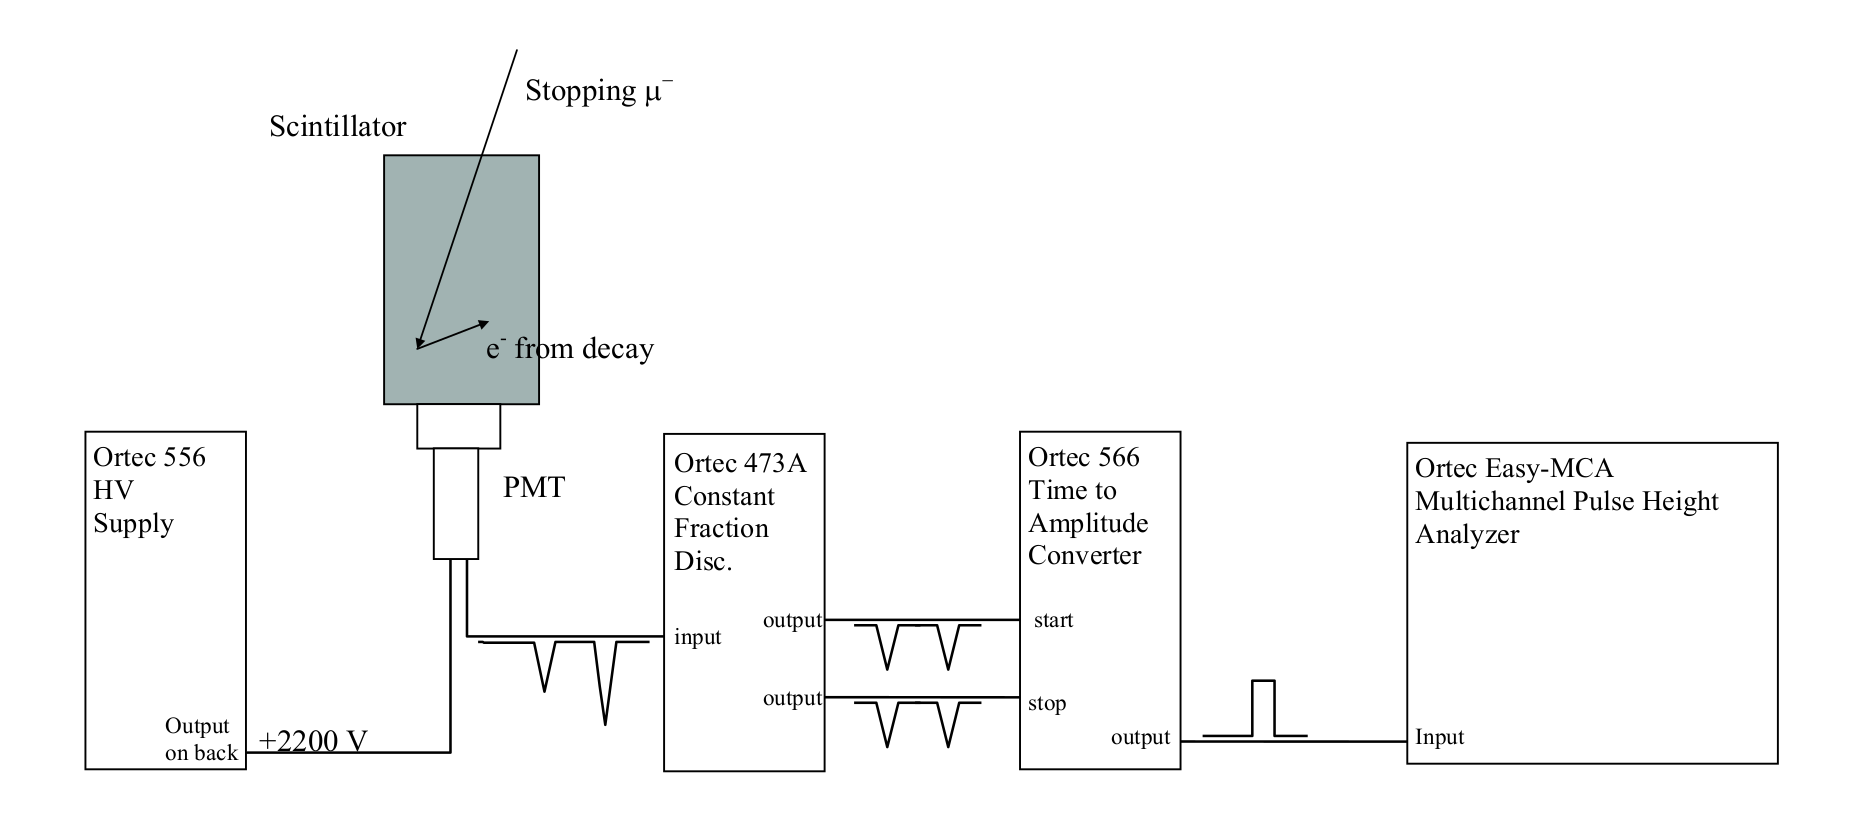
\includegraphics[scale=0.25]{schematic.png}
	\caption{The complete apparatus, consisting of the power supply, scintillator, discriminator, time-to-amplitude converter, and pulse height analyzer. The pulse shapes are shown, conceptually, in the figure. The PMT outputs electron signals from light beams in the scintillator. The CFD filters these signals to reduce noise. The TAC converts the time between pulses to an amplitude. The Pulse Height Analyzer reads the TAC output.\cite{oxymanual}}
\end{figure}

\subsection{Calibration}

Calibration of the apparatus was completed in two steps. First, the CFD was calibrated by using a pulse generator to send of pulses of a fixed amplitude to the CFD. The signal from the pulse generator was connected to the CFD input using a T-connector, which was then routed to the oscilloscope. The CFD was adjusted so that the pulses were output to the screen of the oscilloscope with minimal noise. This process was repeated for various pulse amplitudes in order to find a proper CFD value for differing conditions.

The next step of calibration was for the MCA time scale. The pulse generator was set to output two pulses at a time $\Delta t$ apart. The “measure” menu on the oscilloscope allows for easy measurement of this time separation. These dual pulse signals were then sent to the CFD, which would thus filter the signals based on the time separation, not the amplitude of the pulse. The CFD was set so that the oscilloscope consistently gave an output. The oscilloscope was set for two outputs, one from the CFD and another from the MCA. During a muon decay event, the dual channel oscilloscope setup on the screen looks like two large pulses at a short distance from one another for the CFD output. For the MCA output, this event is one rectangular pulse that varies in amplitude based on the time separation of the CFD pulses.

\subsection{Data Collection}

Collecting data for this experiment was as simple as replacing the input to the CFD (discriminator) from the pulse generator to the PMT from the scintillator box. This allowed for pulses from decaying muons in the box to be collected instead of constant pulses from the generator. The MAESTRO software provided was used to collect counts of decay events occurring in the scintillator box.

Data was collected over the time of about a 72-hour period to allow for a large sample of decay events to be recorded. This large sample period minimizes the uncertainty when calculating the lifetime of the muon due to the increased number of values near the actual lifetime versus outlier values.

\section{\label{sec:level4}Data Analysis}

A long experimental run of 72 hours was run at a CFD value of 1 *to-do:units* and TAC value of *to-do: fill in value*. Figures 2, 3, and 4 are representative of three different sample events captured with the oscilloscope single shot mode. The yellow pulses in the figure represent the actual decay events. The first pulse is the muon creation, followed by a second pulse, the end of life of the muon. The green pulse is the output from the TAC, with an amplitude related to the time-separation of the green pulses. The measured time of decay for these sample events are *to-do:measure these* *, *, and *, respectively.

\begin{figure}[H]
	\centering
	\subfloat{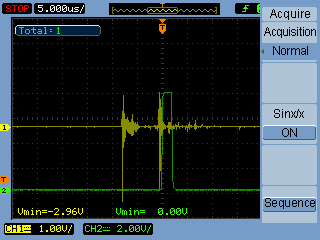
\includegraphics[width=2.3in]{A.png}}\hfill
	\subfloat{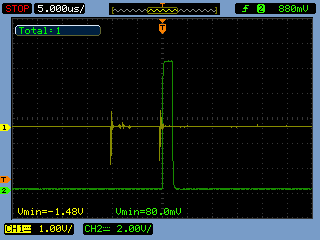
\includegraphics[width=2.3in]{B.png}}\hfill
	\subfloat{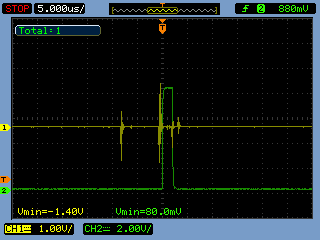
\includegraphics[width=2.3in]{C.png}}
	\caption{Sample muon decay events, taken with the oscilloscope single shot mode.}
\end{figure}

The histogram captured from the MAESTRO software is shown in Figure 3. The data was exported in ASCII format and uploaded into Microsoft Excel for analysis. *to-do: explain channel time width*
% 500 channels
% 100 nanoseconds
% 100 multiplier
% 0.05 microseconds per channel
% 2.2 seconds is around channel 110

% singles rate:
% 1200 for one minute
% according to wikipedia: should get 600 per minute for a box of 0.05% size of 1m^2

\begin{figure}[H]
	\centering
	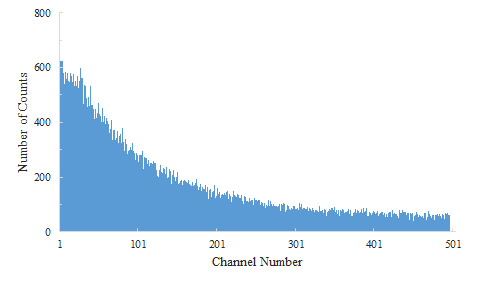
\includegraphics[scale=0.8]{unfiltered.png}
	\caption{The histogram of counts for pulse events where pulses are only detected if their amplitude is above the discriminator trigger value.}
\end{figure}

In Figure 3, there is a point where the decay curve flattens out into the “background". The background is due to discriminator pulses randomly occurring above the trigger value that was set. Channels 221 to 500 were averaged to conclude a background value of 78.8. This background was subtracted from the decay curve (channels 0 to 220) and shown in Figure 4. A best-fit line was applied to the filtered data, providing a slope of $-2.25 \pm 0.04$ \textmu s. The standard error of the slope was provided by applying a regression analysis to the data.

\begin{figure}[H]
	\centering
	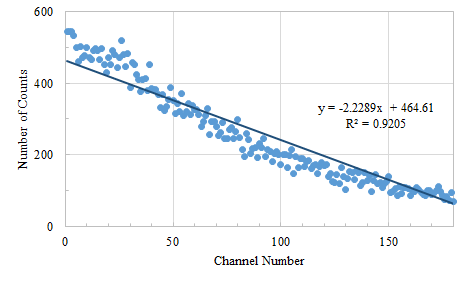
\includegraphics[scale=0.8]{filtered.png}
	\caption{After the background has been subtracted from the histogram, the following is left over. The slope of the best-fit line represents the lifetime of the muon.}
\end{figure}

\section{\label{sec:level5}Conclusion}


\nocite{*}
\bibliography{main}% Produces the bibliography via BibTeX.
\end{document}
